\begin{center}
\footnotesize\noindent\fbox{
	\parbox{\textwidth}{
	Stimare, nel senso dei minimi quadrati, posizione, velocit\'a iniziale ed accelerazione relative ad un moto rettilineo uniformemente accelerato per cui sono note le seguenti misurazioni dele coppie \((tempo, spazio)\):\\
	\((1, 2.9) \quad (1, 3.1)\quad (2, 6.9) \quad (2, 7.1) \quad (3, 12.9) \quad (3, 13.1) \quad (4, 20.9) \quad (4, 21.1) \quad (5, 30.9) \quad (5, 31.1)\)
	}
}\end{center}

\noindent La legge che descrive il fenomeno del moto rettilineo uniformemente accelerato (in realt\'a ben nota, come vedremo) \'e di tipo polinomiale, e mette in relazione due grandezze sperimentali quali un intervallo di tempo ed uno spostamento. Si ricerca quindi il polinomio che meglio approssima le coppie di dati fornite, nel senso di nei minimi quadrati. 

\noindent Ricordando che possiamo esprimere la coordinata spaziale della dimensione che ci interessa in funzione del tempo trascorso da un certo istante zero, abbiamo che:

\[
  y =  s(t) = x_0 + v_0t + \frac{1}{2}at^2 \quad \quad \text{con } a \text{, } x_0 \text{ e } v_0 \text{ costanti}
\]

\noindent Il polinomio interpolante tale legge fisica avr\'a la seguente forma:

\[
  y = \sum^m_{k=0}a_kx^k
\]

\noindent con il vettore dei coefficienti \textbf{a} tale da minimizzare la quantit\'a \(||\textbf{y}-\textbf{z}||^2_2 = \sum^n_{i=0}|y_i-z_i|^2\), ed il vettore \textbf{z} definito come segue:

\[
  \textbf{z} = \begin{pmatrix} \sum_{k=0}^m a_kx_0^k \\ \vdots \\  \sum_{k=0}^m a_kx_n^k \end{pmatrix} = V \textbf{a}
\]

\noindent Si tratta quindi di risolvere il sistema sovradeterminato \(V \textbf{a} = \textbf{y} \), con \(V\) matrice di tipo Vandermonde.
\\ \\
\noindent Le coppie di dati fornite sono del tipo \((x, y) \equiv  (tempo, spazio)\) e sono state usate nel seguente codice Matlab per trovare e plottare il miglior polinomio approssimante di secondo grado:

\begin{center}
	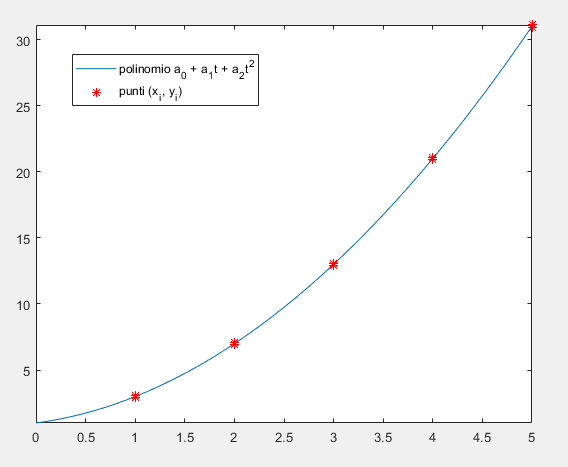
\includegraphics[scale=0.6]{cap4/4_10.png}
\end{center}

\lstinputlisting[language=Matlab]{cap4/4_10.m}
\vspace{0.2cm}
\noindent Essendo il polinomio interpolante \(p(t) = 1 + t + t^2\) perfettamente analogo alla legge fisica \(s(t) = x_0 + v_0t + \frac{1}{2}at^2\), abbiamo banalmente i seguenti valori per  posizione iniziale, velocit\'a iniziale ed accelerazione:

\[
  x_0 = 1
\]
\[
  v_0 = 1
\]
\[
  a = 1
\]
